\documentclass[twoside]{book}

% Packages required by doxygen
\usepackage{fixltx2e}
\usepackage{calc}
\usepackage{doxygen}
\usepackage[export]{adjustbox} % also loads graphicx
\usepackage{graphicx}
\usepackage[utf8]{inputenc}
\usepackage{makeidx}
\usepackage{multicol}
\usepackage{multirow}
\PassOptionsToPackage{warn}{textcomp}
\usepackage{textcomp}
\usepackage[nointegrals]{wasysym}
\usepackage[table]{xcolor}

% Font selection
\usepackage[T1]{fontenc}
\usepackage[scaled=.90]{helvet}
\usepackage{courier}
\usepackage{amssymb}
\usepackage{sectsty}
\renewcommand{\familydefault}{\sfdefault}
\allsectionsfont{%
  \fontseries{bc}\selectfont%
  \color{darkgray}%
}
\renewcommand{\DoxyLabelFont}{%
  \fontseries{bc}\selectfont%
  \color{darkgray}%
}
\newcommand{\+}{\discretionary{\mbox{\scriptsize$\hookleftarrow$}}{}{}}

% Page & text layout
\usepackage{geometry}
\geometry{%
  a4paper,%
  top=2.5cm,%
  bottom=2.5cm,%
  left=2.5cm,%
  right=2.5cm%
}
\tolerance=750
\hfuzz=15pt
\hbadness=750
\setlength{\emergencystretch}{15pt}
\setlength{\parindent}{0cm}
\setlength{\parskip}{3ex plus 2ex minus 2ex}
\makeatletter
\renewcommand{\paragraph}{%
  \@startsection{paragraph}{4}{0ex}{-1.0ex}{1.0ex}{%
    \normalfont\normalsize\bfseries\SS@parafont%
  }%
}
\renewcommand{\subparagraph}{%
  \@startsection{subparagraph}{5}{0ex}{-1.0ex}{1.0ex}{%
    \normalfont\normalsize\bfseries\SS@subparafont%
  }%
}
\makeatother

% Headers & footers
\usepackage{fancyhdr}
\pagestyle{fancyplain}
\fancyhead[LE]{\fancyplain{}{\bfseries\thepage}}
\fancyhead[CE]{\fancyplain{}{}}
\fancyhead[RE]{\fancyplain{}{\bfseries\leftmark}}
\fancyhead[LO]{\fancyplain{}{\bfseries\rightmark}}
\fancyhead[CO]{\fancyplain{}{}}
\fancyhead[RO]{\fancyplain{}{\bfseries\thepage}}
\fancyfoot[LE]{\fancyplain{}{}}
\fancyfoot[CE]{\fancyplain{}{}}
\fancyfoot[RE]{\fancyplain{}{\bfseries\scriptsize Generated by Doxygen }}
\fancyfoot[LO]{\fancyplain{}{\bfseries\scriptsize Generated by Doxygen }}
\fancyfoot[CO]{\fancyplain{}{}}
\fancyfoot[RO]{\fancyplain{}{}}
\renewcommand{\footrulewidth}{0.4pt}
\renewcommand{\chaptermark}[1]{%
  \markboth{#1}{}%
}
\renewcommand{\sectionmark}[1]{%
  \markright{\thesection\ #1}%
}

% Indices & bibliography
\usepackage{natbib}
\usepackage[titles]{tocloft}
\setcounter{tocdepth}{3}
\setcounter{secnumdepth}{5}
\makeindex

% Hyperlinks (required, but should be loaded last)
\usepackage{ifpdf}
\ifpdf
  \usepackage[pdftex,pagebackref=true]{hyperref}
\else
  \usepackage[ps2pdf,pagebackref=true]{hyperref}
\fi
\hypersetup{%
  colorlinks=true,%
  linkcolor=blue,%
  citecolor=blue,%
  unicode%
}

% Custom commands
\newcommand{\clearemptydoublepage}{%
  \newpage{\pagestyle{empty}\cleardoublepage}%
}

\usepackage{caption}
\captionsetup{labelsep=space,justification=centering,font={bf},singlelinecheck=off,skip=4pt,position=top}

%===== C O N T E N T S =====

\begin{document}

% Titlepage & ToC
\hypersetup{pageanchor=false,
             bookmarksnumbered=true,
             pdfencoding=unicode
            }
\pagenumbering{alph}
\begin{titlepage}
\vspace*{7cm}
\begin{center}%
{\Large Timer Driver \\[1ex]\large Version 1.\+0.\+0 }\\
\vspace*{1cm}
{\large Generated by Doxygen 1.8.13}\\
\end{center}
\end{titlepage}
\clearemptydoublepage
\pagenumbering{roman}
\tableofcontents
\clearemptydoublepage
\pagenumbering{arabic}
\hypersetup{pageanchor=true}

%--- Begin generated contents ---
\chapter{Timer Driver\+: An adventure}
\label{md__home_marko__documents_embedded_workspace_timer_driver__r_e_a_d_m_e}
\Hypertarget{md__home_marko__documents_embedded_workspace_timer_driver__r_e_a_d_m_e}
This driver took a bit more creative thinking to be able to combine both regular timer usage and more complex compare/capture usage into a single interface. Of course it became two interfaces, the timer\+\_\+interface and timer\+\_\+cc\+\_\+interface. An extra challenge was thinking through how to get the exact same driver to work for the three different types of timers on the stm32\+F411\+XE. The answer was to work around the weakest ones (T\+I\+M10 and T\+I\+M11). All fancy advanced features of T\+I\+M1 must be accessed the hard way with register reads and writes. 
\chapter{Data Structure Index}
\section{Data Structures}
Here are the data structures with brief descriptions\+:\begin{DoxyCompactList}
\item\contentsline{section}{\hyperlink{structtimer__advanced__t}{timer\+\_\+advanced\+\_\+t} }{\pageref{structtimer__advanced__t}}{}
\item\contentsline{section}{\hyperlink{structtimer__cc__config__t}{timer\+\_\+cc\+\_\+config\+\_\+t} }{\pageref{structtimer__cc__config__t}}{}
\item\contentsline{section}{\hyperlink{structtimer__config__t}{timer\+\_\+config\+\_\+t} }{\pageref{structtimer__config__t}}{}
\item\contentsline{section}{\hyperlink{structtimer__external__trigger__t}{timer\+\_\+external\+\_\+trigger\+\_\+t} }{\pageref{structtimer__external__trigger__t}}{}
\end{DoxyCompactList}

\chapter{Data Structure Documentation}
\hypertarget{structtimer__advanced__t}{}\section{timer\+\_\+advanced\+\_\+t Struct Reference}
\label{structtimer__advanced__t}\index{timer\+\_\+advanced\+\_\+t@{timer\+\_\+advanced\+\_\+t}}


Collaboration diagram for timer\+\_\+advanced\+\_\+t\+:\nopagebreak
\begin{figure}[H]
\begin{center}
\leavevmode
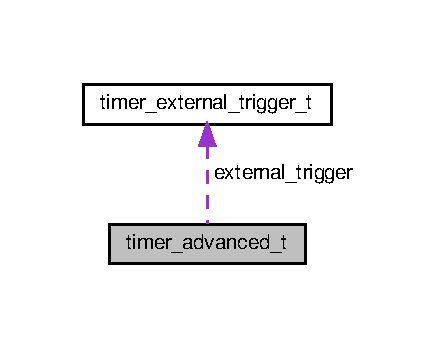
\includegraphics[width=210pt]{structtimer__advanced__t__coll__graph}
\end{center}
\end{figure}
\subsection*{Data Fields}
\begin{DoxyCompactItemize}
\item 
\mbox{\Hypertarget{structtimer__advanced__t_af18601db6c5fffc07d7d214c606f2f00}\label{structtimer__advanced__t_af18601db6c5fffc07d7d214c606f2f00}} 
timer\+\_\+opm\+\_\+t {\bfseries one\+\_\+pulse\+\_\+mode}
\item 
\mbox{\Hypertarget{structtimer__advanced__t_acebb1b98929e7dd770f19b5448ccfe95}\label{structtimer__advanced__t_acebb1b98929e7dd770f19b5448ccfe95}} 
timer\+\_\+udis\+\_\+t {\bfseries update\+\_\+event\+\_\+dis}
\item 
\mbox{\Hypertarget{structtimer__advanced__t_a9dc93b02cbfef454d4e6018065e03990}\label{structtimer__advanced__t_a9dc93b02cbfef454d4e6018065e03990}} 
timer\+\_\+trigger\+\_\+t {\bfseries trigger}
\item 
\mbox{\Hypertarget{structtimer__advanced__t_a4c82d8472fb549c1b19979f124b4c10f}\label{structtimer__advanced__t_a4c82d8472fb549c1b19979f124b4c10f}} 
const \hyperlink{structtimer__external__trigger__t}{timer\+\_\+external\+\_\+trigger\+\_\+t} $\ast$ {\bfseries external\+\_\+trigger}
\end{DoxyCompactItemize}


The documentation for this struct was generated from the following file\+:\begin{DoxyCompactItemize}
\item 
/home/marko/\+Documents/embedded\+\_\+workspace/timer\+\_\+driver/timer\+\_\+stm32f411\+\_\+config.\+h\end{DoxyCompactItemize}

\hypertarget{structtimer__cc__config__t}{}\section{timer\+\_\+cc\+\_\+config\+\_\+t Struct Reference}
\label{structtimer__cc__config__t}\index{timer\+\_\+cc\+\_\+config\+\_\+t@{timer\+\_\+cc\+\_\+config\+\_\+t}}
\subsection*{Data Fields}
\begin{DoxyCompactItemize}
\item 
\mbox{\Hypertarget{structtimer__cc__config__t_aa1903ec0ba4500a4e29acd8791a6d4cc}\label{structtimer__cc__config__t_aa1903ec0ba4500a4e29acd8791a6d4cc}} 
timer\+\_\+cc\+\_\+mode\+\_\+t {\bfseries cc\+\_\+mode}
\item 
\mbox{\Hypertarget{structtimer__cc__config__t_a0a5da7bca402a4196c5edd12329cb965}\label{structtimer__cc__config__t_a0a5da7bca402a4196c5edd12329cb965}} 
timer\+\_\+cc\+\_\+output\+\_\+polarity\+\_\+t {\bfseries output\+\_\+polarity}
\item 
\mbox{\Hypertarget{structtimer__cc__config__t_a7b3472060b75968f2686db112b700530}\label{structtimer__cc__config__t_a7b3472060b75968f2686db112b700530}} 
timer\+\_\+cc\+\_\+output\+\_\+fe\+\_\+t {\bfseries output\+\_\+fast\+\_\+enable}
\item 
\mbox{\Hypertarget{structtimer__cc__config__t_ad392f1537a58c13a98a5c76f6019cfa2}\label{structtimer__cc__config__t_ad392f1537a58c13a98a5c76f6019cfa2}} 
timer\+\_\+cc\+\_\+output\+\_\+pe\+\_\+t {\bfseries output\+\_\+preload\+\_\+enable}
\item 
\mbox{\Hypertarget{structtimer__cc__config__t_a5f9f6841dbd86558517bb472b4daad88}\label{structtimer__cc__config__t_a5f9f6841dbd86558517bb472b4daad88}} 
timer\+\_\+cc\+\_\+output\+\_\+mode\+\_\+t {\bfseries output\+\_\+mode}
\item 
\mbox{\Hypertarget{structtimer__cc__config__t_a87dbba1714ff844cdf36ae87a3a86e19}\label{structtimer__cc__config__t_a87dbba1714ff844cdf36ae87a3a86e19}} 
timer\+\_\+cc\+\_\+output\+\_\+ce\+\_\+t {\bfseries output\+\_\+clear\+\_\+enable}
\item 
\mbox{\Hypertarget{structtimer__cc__config__t_ab7cf4de41a7ee3ee78bb9999f2092565}\label{structtimer__cc__config__t_ab7cf4de41a7ee3ee78bb9999f2092565}} 
timer\+\_\+cc\+\_\+input\+\_\+prescaler\+\_\+t {\bfseries input\+\_\+event\+\_\+prescaler}
\item 
\mbox{\Hypertarget{structtimer__cc__config__t_ac2cab03b6d1e6c64bb83eb0a78f08391}\label{structtimer__cc__config__t_ac2cab03b6d1e6c64bb83eb0a78f08391}} 
timer\+\_\+cc\+\_\+input\+\_\+filter\+\_\+t {\bfseries input\+\_\+event\+\_\+filter}
\item 
\mbox{\Hypertarget{structtimer__cc__config__t_ace0c49b91c2083d06b4bbd59c5eab9fb}\label{structtimer__cc__config__t_ace0c49b91c2083d06b4bbd59c5eab9fb}} 
timer\+\_\+cc\+\_\+input\+\_\+polarity\+\_\+t {\bfseries input\+\_\+polarity}
\end{DoxyCompactItemize}


The documentation for this struct was generated from the following file\+:\begin{DoxyCompactItemize}
\item 
/home/marko/\+Documents/embedded\+\_\+workspace/timer\+\_\+driver/timer\+\_\+cc\+\_\+stm32f411\+\_\+config.\+h\end{DoxyCompactItemize}

\hypertarget{structtimer__config__t}{}\section{timer\+\_\+config\+\_\+t Struct Reference}
\label{structtimer__config__t}\index{timer\+\_\+config\+\_\+t@{timer\+\_\+config\+\_\+t}}


Collaboration diagram for timer\+\_\+config\+\_\+t\+:\nopagebreak
\begin{figure}[H]
\begin{center}
\leavevmode
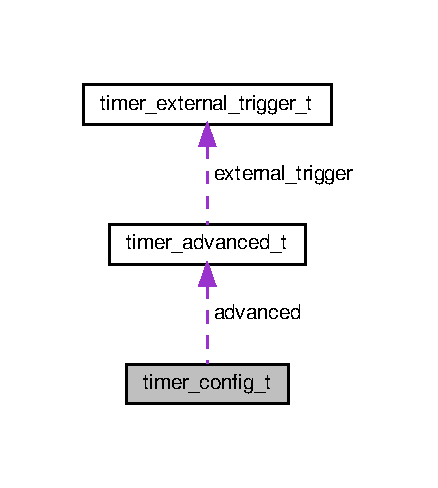
\includegraphics[width=210pt]{structtimer__config__t__coll__graph}
\end{center}
\end{figure}
\subsection*{Data Fields}
\begin{DoxyCompactItemize}
\item 
\mbox{\Hypertarget{structtimer__config__t_afcad5c326fbc98732a2849a5225d8a10}\label{structtimer__config__t_afcad5c326fbc98732a2849a5225d8a10}} 
timer\+\_\+clock\+\_\+source\+\_\+t {\bfseries clock\+\_\+source}
\item 
\mbox{\Hypertarget{structtimer__config__t_ad1aebaa930fb024d94829b73b1cef3a1}\label{structtimer__config__t_ad1aebaa930fb024d94829b73b1cef3a1}} 
timer\+\_\+slave\+\_\+mode\+\_\+t {\bfseries slave\+\_\+mode}
\item 
\mbox{\Hypertarget{structtimer__config__t_ae59142bc6d98c07daf92bb4a0a863d5d}\label{structtimer__config__t_ae59142bc6d98c07daf92bb4a0a863d5d}} 
timer\+\_\+alignment\+\_\+t {\bfseries alignment}
\item 
\mbox{\Hypertarget{structtimer__config__t_a2302b90b0b06bc1915986e83fbec6eb0}\label{structtimer__config__t_a2302b90b0b06bc1915986e83fbec6eb0}} 
timer\+\_\+direction\+\_\+t {\bfseries direction}
\item 
\mbox{\Hypertarget{structtimer__config__t_aec4b74e5d98386ca6cef3847203f8e32}\label{structtimer__config__t_aec4b74e5d98386ca6cef3847203f8e32}} 
timer\+\_\+prescaler\+\_\+t {\bfseries prescaler}
\item 
\mbox{\Hypertarget{structtimer__config__t_a6103ecdcf646d403714e19d5642243b3}\label{structtimer__config__t_a6103ecdcf646d403714e19d5642243b3}} 
uint32\+\_\+t {\bfseries auto\+\_\+reload}
\item 
\mbox{\Hypertarget{structtimer__config__t_a0464cd79f525a0c6d78838e4bc7e50e9}\label{structtimer__config__t_a0464cd79f525a0c6d78838e4bc7e50e9}} 
timer\+\_\+arpe\+\_\+t {\bfseries auto\+\_\+reload\+\_\+preload\+\_\+en}
\item 
\mbox{\Hypertarget{structtimer__config__t_afca478eacfee9c81af1cacb1c3e45195}\label{structtimer__config__t_afca478eacfee9c81af1cacb1c3e45195}} 
const \hyperlink{structtimer__advanced__t}{timer\+\_\+advanced\+\_\+t} $\ast$ {\bfseries advanced}
\end{DoxyCompactItemize}


The documentation for this struct was generated from the following file\+:\begin{DoxyCompactItemize}
\item 
/home/marko/\+Documents/embedded\+\_\+workspace/timer\+\_\+driver/timer\+\_\+stm32f411\+\_\+config.\+h\end{DoxyCompactItemize}

\hypertarget{structtimer__external__trigger__t}{}\section{timer\+\_\+external\+\_\+trigger\+\_\+t Struct Reference}
\label{structtimer__external__trigger__t}\index{timer\+\_\+external\+\_\+trigger\+\_\+t@{timer\+\_\+external\+\_\+trigger\+\_\+t}}
\subsection*{Data Fields}
\begin{DoxyCompactItemize}
\item 
\mbox{\Hypertarget{structtimer__external__trigger__t_a27a62b19d6a850e47d8ebe8a707d49f2}\label{structtimer__external__trigger__t_a27a62b19d6a850e47d8ebe8a707d49f2}} 
timer\+\_\+external\+\_\+trigger\+\_\+filter\+\_\+t {\bfseries filter}
\item 
\mbox{\Hypertarget{structtimer__external__trigger__t_a50a2ed67206a967be3a10af1b4685cce}\label{structtimer__external__trigger__t_a50a2ed67206a967be3a10af1b4685cce}} 
timer\+\_\+external\+\_\+trigger\+\_\+prescaler\+\_\+t {\bfseries prescaler}
\item 
\mbox{\Hypertarget{structtimer__external__trigger__t_acb707cdb7947ed2346965b26bb418c45}\label{structtimer__external__trigger__t_acb707cdb7947ed2346965b26bb418c45}} 
timer\+\_\+external\+\_\+trigger\+\_\+polarity\+\_\+t {\bfseries polarity}
\end{DoxyCompactItemize}


The documentation for this struct was generated from the following file\+:\begin{DoxyCompactItemize}
\item 
/home/marko/\+Documents/embedded\+\_\+workspace/timer\+\_\+driver/timer\+\_\+stm32f411\+\_\+config.\+h\end{DoxyCompactItemize}

%--- End generated contents ---

% Index
\backmatter
\newpage
\phantomsection
\clearemptydoublepage
\addcontentsline{toc}{chapter}{Index}
\printindex

\end{document}
